\pagestyle{fancy}
\headheight 20pt
\lhead{Ph.D. Thesis --- R. Woods }
\rhead{McMaster - Physics \& Astronomy}
\chead{}
\lfoot{}
\cfoot{\thepage}
\rfoot{}
\renewcommand{\headrulewidth}{0.1pt}
\renewcommand{\footrulewidth}{0.1pt}

\chapter{Applications to Galaxy Formation and Future Projects}
\label{chap:galaxyformation}
\thispagestyle{fancy}

We now use the algorithm described in chapter \ref{chap:method} and tested in chapter \ref{chap:codetests} to carry out simulations of an isolated galaxy. We have chosen to start with an isolated galaxy in order to probe the FUV field present in a [Milky Way-like... z=1?] disk in order to check if it is an important SF regulation mechanism.

FUV is an interesting band to start with for a few reasons. While FUV does not ionize gas, it is the primary driver of photoelectric heating \citep{tielens05}, which is the dominant heating mechanism for the ISM and the warm neutral medium. Despite this, very few astrophysical simulations actually include photoelectric heating due to its dependence on a radiation field.

As well, FUV is typically able to penetrate further into the ISM. At common densities in the ISM, an optical depth of 1 is typically only achieved after roughly one kpc. Current simulations, especially of isolated galaxies, can resolve distances much smaller than this, so looking at effects due to FUV is very feasible. On the other hand, bands such as EUV are usually absorbed within a few pc, a resolution that is very costly for even isolated galaxy simulations.

We have chosen to use an isolated galaxy IC from the AGORA galaxy comparison project \citep{kimEt14} to ensure use of a well-tested IC and provide a larger base for comparison of results.

\section{FUV Fields in the AGORA Disk}
\label{sec:agora}

The AGORA galaxy comparison project is a large computational comparison project that aims ``to raise the realism and predictive power of galaxy simulations and the understanding of the feedback processes that regulate galaxy `metabolism,' and by doing so to solve long-standing problems in galaxy formation'' \citep{kimEt14}. To accomplish this, the project has created both isolated and cosmological galaxy formation initial conditions at many different masses and resolutions, and has attempted to standardize physics modules and analysis methods for all of the codes involved in the project.

\subsection{Initial Conditions and Physics}
\label{sec:initialconditions}

We have chosen to run the isolated disk initial condition in order to examine FUV's effect on the ISM. The specific details of the ICs for this disk can be found in \citet{kimEt14}, section 2.2. We summarize here the important information.

The initial conditions have been generated at three different resolutions using the \textsc{MakeDisk} code, written by Volker Springel. The disk is created with four components: a dark matter halo, a gas disk, a stellar disk, and stellar bulge. The low resolution disk has $10^5$ DM particles, $10^5$ stellar disk particles, $10^5$ gas particles, and $1.24\e{4}$ stellar bulge particles. The medium and high resolution disks have 10 and 100 times more particles in each component, respectively.

The DM follows a NFW profile \citep{navarroEt97} with a concentration parameter $c = 10$ and a spin parameter $\lambda = 0.04$. The disk has an exponential profile with a scale length of $r_d = 3.432$ kpc and a scale height of $z_d = 0.1 r_d$. The disk is split into the stellar component, which has a mass of $4.297\e{10} M_{\odot}$, and a gas component, which has a mass of 20\% of the DM mass. The stellar bulge follows the Hernquist \citeyear{hernquist90} density profile with a bulge-to-disk mass ratio of B/D = 0.1. Gas is initiated at $10^4$ K. The \textsc{MakeDisk} code ensures that the above conditions give quasi-equilibrium [what does that mean?] for the four components. An image of the IC is shown in figure \ref{fig:agoraic}.

\begin{figure}

\includegraphics[width=\textwidth]{graphics/placeholder.eps}
\caption[The AGORA IC]{A density slice in the z plane of the AGORA initial condition.}
\label{fig:agoraic}
\end{figure}

%notes about various runs we did

We have run the low resolution simulation with a number of different physical parameters, including our radiative transfer with FUV, a background FUV at two intensities (the standard for most codes without radiative transfer), and Supernovae (SNe) feedback \citep{kellerEt14}. Table \ref{tab:simsummary} summarizes the simulations and the names we have given them.

\begin{table}
\begin{tabular}{llll}
Name & RT & UV Strength (units?) & SNe Feedback\\ \hline \hline
RadFUV & Yes & 0 & No\\
RadFUV2e-26 & No & 2e-26 & No\\
RadFUV2e-27 & No & 2e-27 & No\\
RadFB & No & ? & yes\\
RadFB\_FUV & Yes & 0 & yes\\
RadFB\_FUV2e-26 & No & 2e-26 & yes\\
RadFB\_FUV2-27 & No & 2e-27 & yes\\
\hline
\end{tabular}
\caption[Summary of simulations]{A summary of the simulations that were run.}
\end{table}

We have also included a run at medium resolution to check on convergence of results. It is important to note that resolution may play an important factor in the following results. \citet{FILL IN} [ask sam for references] found that in order to get proper ISM behavior, a simulation needs to be at a high enough resolution. As will be noted in section \ref{sec:futurework}, a convergence study in resolution should be performed on this work.

\section{The Role of FUV on Star Formation}
\label{sec:fuvsfr}


We begin by looking at the star formation history of each simulation. Figure \ref{fig:sfrvtime} shows the star formation rate as a function of time for each simulation. 

\begin{figure}
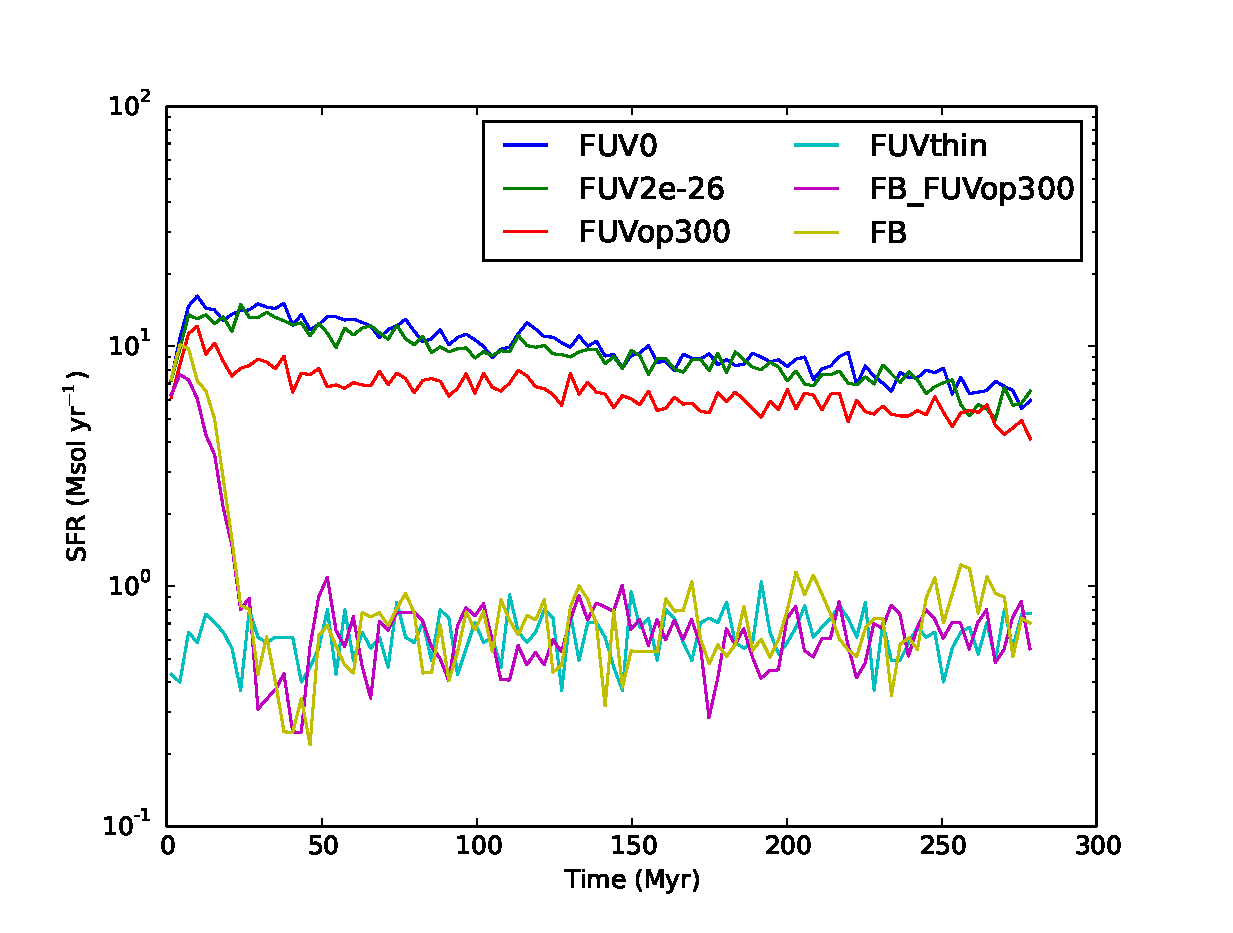
\includegraphics[width=\textwidth]{graphics/sfrvtime.eps}
\caption[Star formation histories.]{Star formation rate vs time for each simulation. Feedback dominates the star formation regulation in this galaxy. Looking only at FUV, local feedback has a noticeable effect over a uniform background UV field.}
\label{fig:sfrvtime}
\end{figure}

It is clear that SNe feedback has a very strong regulation effect on star formation, as the rate in all runs with SNe feedback is about a factor of five lower than simulations without SNe feedback. In runs without SNe feedback, local FUV fields tend to reduce star formation rates by a factor of around 25\% compared to uniform backgrounds. Comparing the RadFUV2e-26 and RadFUV2e-27, there is no noticeable difference, suggesting that the FUV due to a uniform background has no ability to regulate star formation.

We must check whether the FUV field present in the galaxy is similar to observations. Figure \ref{fig:intensitywolfire} is a plot of FUV intensity vs radius in the midplane of the galaxy.

\begin{figure}
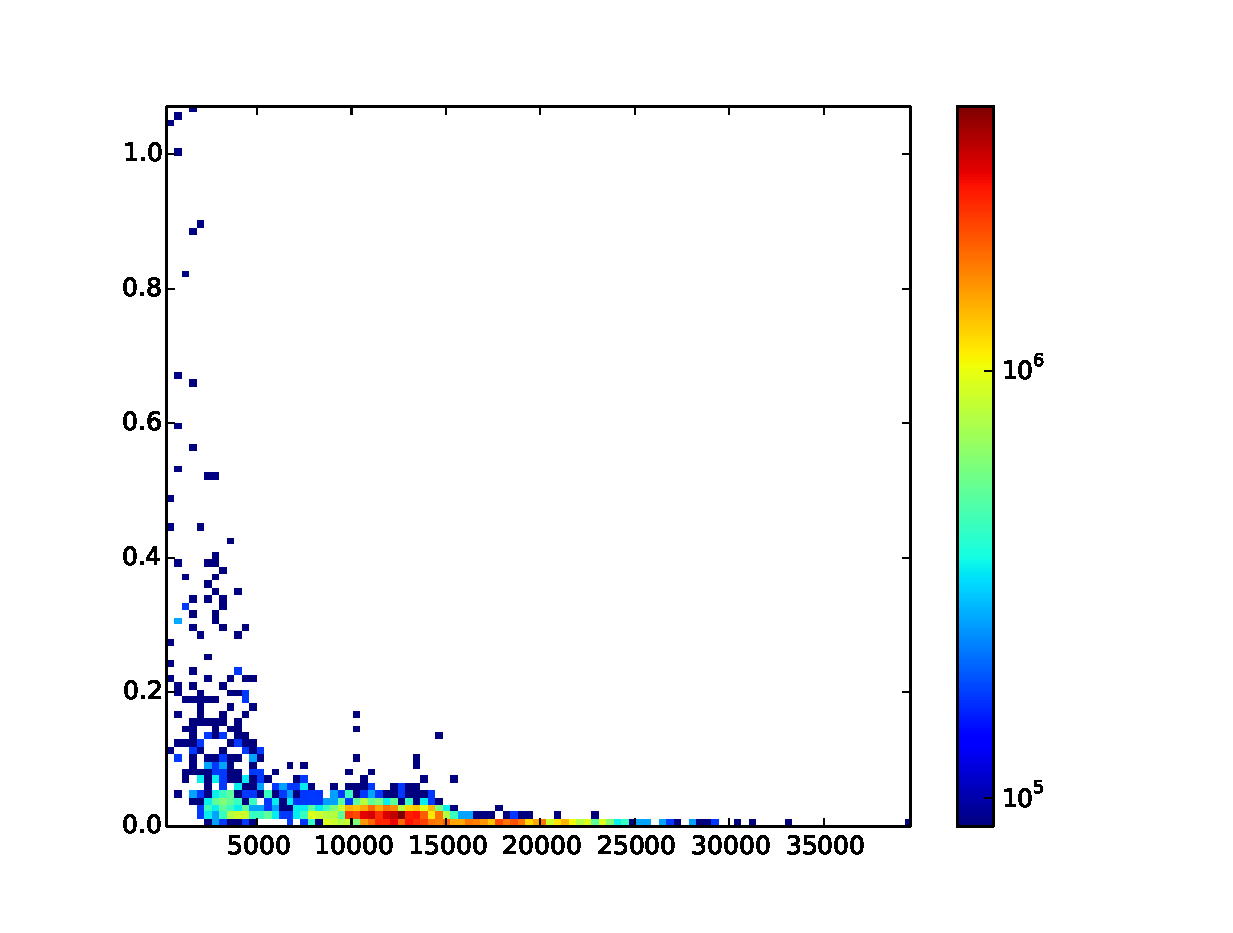
\includegraphics[width=\textwidth]{graphics/intensityvrRadFB_FUV00101.eps}
\caption[FUV intensity vs radius]{FUV intensity vs radius in the galaxy midplane for the RadFUV case. The dots are individual particle fluxes and the solid line is from figure 5.5 of \citet{wolfireEt03}.}
\label{fig:intensitywolfire}
\end{figure}

The points are intensities for individual particles and the lines is the mean intensity presented in \citet{wolfireEt03}. On average, the FUV intensity seen by a particle is far lower than the mean field presented by \citet{wolfireEt03}.

In order to understand the affect FUV has on gas, we consider phase diagrams for gas in the galaxy. Figure \ref{fig:phasediagrams} shows phase diagrams of gas in a number of the different simulations.

\begin{figure}
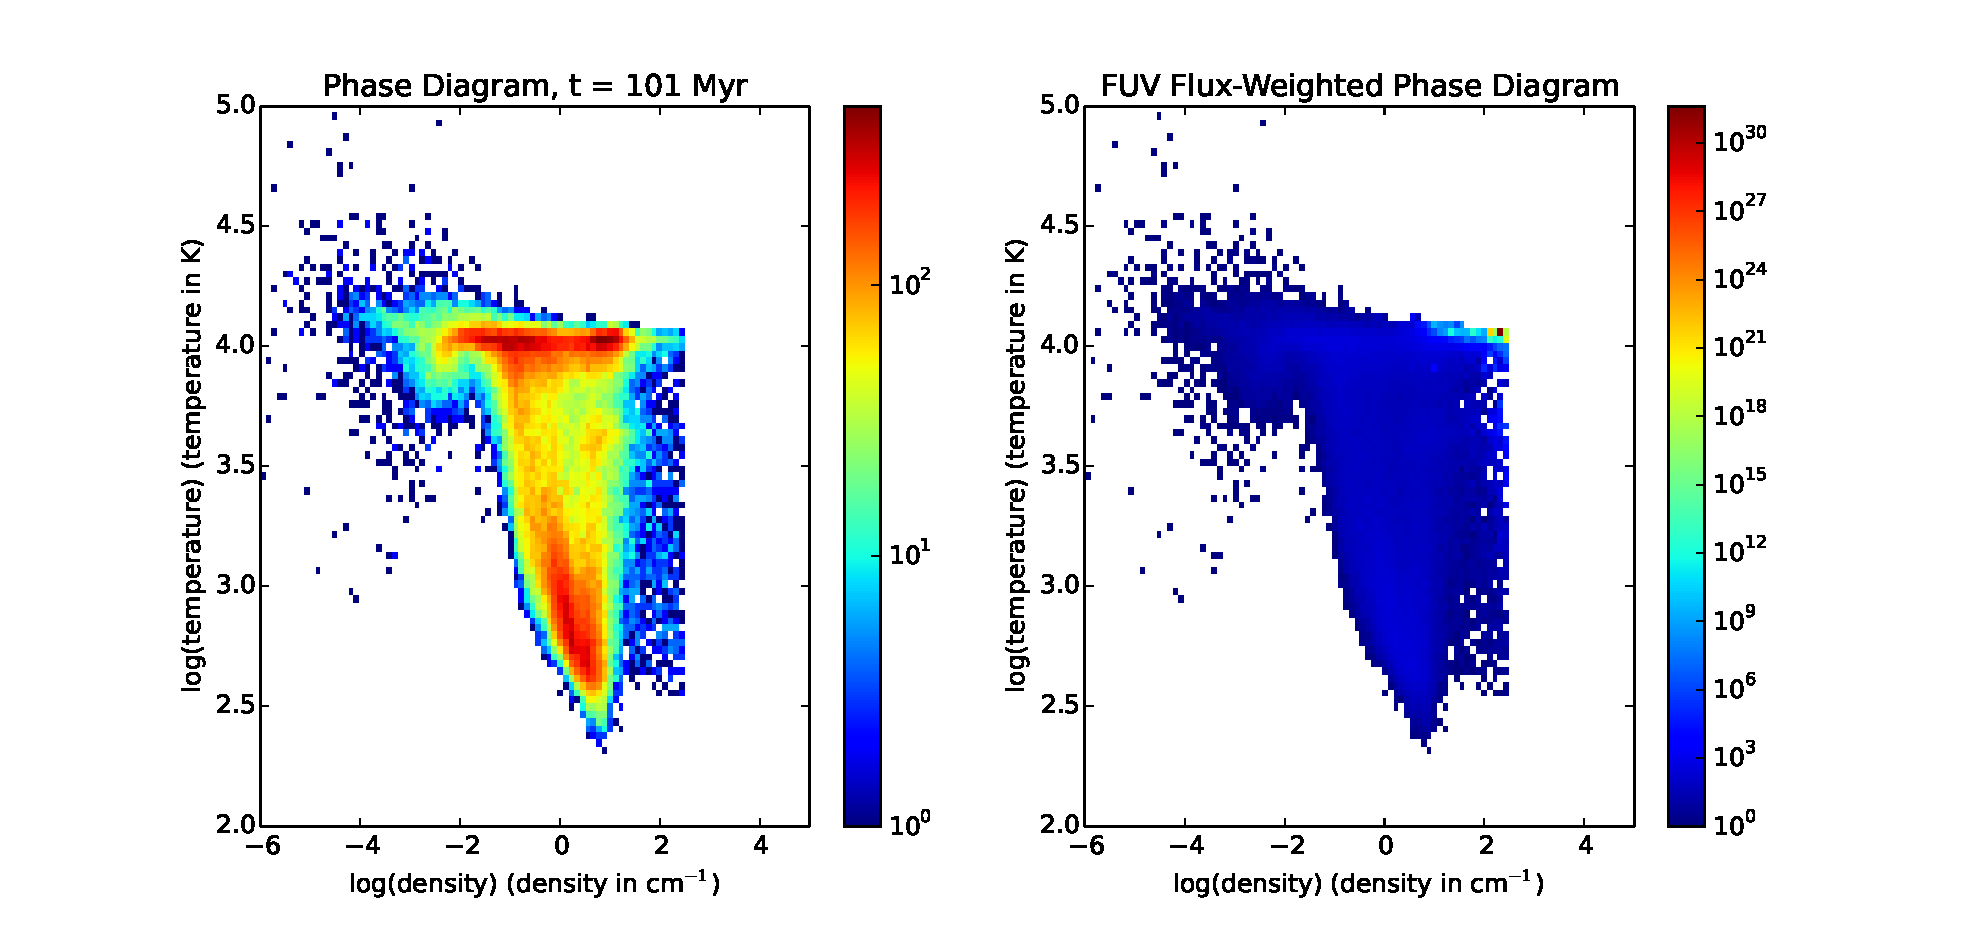
\includegraphics[width=\textwidth]{graphics/phaseRadFUV00101.eps}
\caption[Phase diagrams with different physics]{Phase diagrams for each simulation case.}
\label{fig:phasediagrams}
\end{figure}

In cases with FUV simulated with radiative transfer, a portion of the gas is seen to be heated to about $10^4$ K around densities of 100 atoms cm$^{-3}$.

\section{Future Projects [Move to Ch 6?]}
\label{sec:futurework}

\subsection{Astrophysics Projects}
\label{sec:astroprojects}

Future work of this algorithm is quite broad; the flexibility allows application to a wide range of problems. An immediate follow up is to the work presented in section \ref{sec:agora}. [Author] suggests that four radiation bands, HI ionization, He ionization, LyWerner, and CI, are needed to sufficiently recreate ISM properties. Using these four bands, we would like to calculate the effect of radiation on the ISM. Including these four sources of heating and ionization will enable classification of which bands regulate star formation as a function of environment, and which bands drive particular phases of the ISM.

Currently, there is very little work in computational astrophysics that models the UV fields in and around galaxies. While many models have been created from the observational side [references], due to large computational cost, simulations have left this area largely unexplored or explored only at high redshift [references].

The next project for the radiative transfer code will be to include UV in the McMaster Unbiased Galaxy Simulations 2 (MUGS2) simulations. The MUGS2 project is a set of cosmological simulations of galaxies spanning a large range of parameter space. There are currently [16] galaxies in the set spanning a mass range of $5\e{11} M_{\odot}$ to $2\e{12} M_{\odot}$. Including explicit radiative transfer in these cosmological simulations all the way down to redshift zero would be an unprecedented accomplishment in computational galaxy formation. The group of simulations would enable comparison of the effectiveness of radiative transfer in transforming and regulating galaxy formation across a wide mass range at different epochs in time.

Having a wide range of simulated galaxies all with RT will also enable a plethora of other analysis. Currently, escape fractions of radiation from galaxies are typically assumed to be certain values (e.g. \citet{kannanEt14}). With the MUGS2 simulations including RT, escape fractions could be explicitly calculated.

\textsc{Gasoline} has a chemical network for molecular Hydrogen (H2) creation and destruction \citep{christensenEt12}, but requires an accurate Lyman-Werner field in order to be used. The new RT can provide this, and enables studies on H2 formation and destruction in galaxies, as well as studies of H2 shielding, self and dust, in molecular clouds. This has the additional advantage of easily being linked to observations.

We note that a potential application is to study cosmic re-ionization. However, this application may not be as ideal. Besides having already received a fair bit of attention from simulators, our code does not explicitly conserve photons and so does not guarantee correct ionization front propagation speeds, which are quite important for studies of cosmic re-ionization.

Finally, an exciting potential application is to look at re-radiation of photons from gas. This could include the effects of gas re-radiating ionizing photons when electrons recombine back to the ground state. This effectively increases the penetration depth of ionizing photons and can have an important effect on the gas in the ISM at particular densities [cite rahmati]. As well, processing of stellar emission down to IR wavelengths could be a very interesting study. However, both of these applications rely on a successful implementation of gas radiation in \textsc{Gasoline}. While in principle the implemented RT can handle any radiation, allowing gas to radiate requires care in that it must be self-consistently tied to the cooling that gas experiences. At first glance, separating cooling and cooling radiation induces a cooling instability and so requires further investigation to be done properly (see section \ref{sec:codeadditions}).

\subsection{Code Additions}
\label{sec:codeadditions}

The algorithm we have presented is very flexible, efficient, and powerful. However, there is a lot of room for improvement in the algorithm and optimizations that can be made.

For example, if it is know a priori that all sources lie outside of the absorbing material, the algorithm can be simplified to run in order $N\log{N}$ time by implementing the algorithm presented in TreeCOL \citep{clarkEt12}. In this scenario, each receiving leaf partitions the rest of the tree into equal areas on the sky (TreeCOL uses the HEALPIX algorithm \citep{gorskiEt05}, but it is not required) during the tree walk. Since an effective size of each cell the leaf interacts with can be calculated, each cell can add its absorption contributions to the proper area on the leaf's sky map.

It is also possible to make optimizations in the tree build process. Currently, the tree is rebuilt for every substep the simulation takes, regardless of how large the time step is. It's possible to simply ``fix'' the tree rather than rebuilding it in cases where particles have not moved by much [cite codes that do this]. Along the same lines, it's also possible to avoid recalculating radiation if the time step is very small. If particles have not moved by much and radiation sources have not been significantly changed, than there is no reason to recalculate the radiation field. This would require flagging of ``unimportant'' regions or including a radiation-set time step in the code. If the code time step was smaller than the radiation time step, then the radiation calculation could be skipped.

Currently, the algorithm supports an arbitrary number of wave bands. However, work is still needed to couple the photons in these bands to cooling and heating processes in the code. Adding this functionality will greatly open up the number of projects the algorithm can be used for.

It would also be very interesting to create the ability to use gas particles as sources. This enables the code to treat re-radiation by gas, dust emission, and potentially even scattering if a gas particle's emission in one band was based on its incident intensity in another band. Due to the excellent scaling with the number of sources that the algorithm provides, this should not be computationally prohibitive. The consideration to make here is how self consistent the cooling is with radiation. For example, if a gas particle emits a certain luminosity in certain bands, but the cooling code integrates out a different cooling rate, energy conservation can be violated, and cooling instabilities in the gas particle can be created [more details here]. This code addition will require special attention to get right.

Other minor features can be added without too much difficulty. For example, radiation is currently not allowed to be periodic. However, there is no reason a tree cell cannot be copied in a similar way to gravitational periodicity (where an offset is simply added to each cell in the tree to represent a periodic copy). As well, it is possible to add dynamical effects due to radiation such as radiation pressure. This simply requires code to be added into the acceleration calculations to use the radiation field information.

[closing statement?]